\section{Introduction}\label{sec:introduction}

Qualitative network models make biological hypotheses executable without
requiring a fully parameterized kinetic description. Models assembled for
related functions may nevertheless differ in organism, curation, initial
condition, or update convention. For computational biology, comparing them
requires more than recognizing similar wiring: one must ask whether the models
can reproduce the same biologically relevant steps and choices under a stated
readout.\cite{ChaouiyaPetriBio2007,Li2006,Fisher2007}

DNA-damage response provides a concrete example. Animal/human and
\tas{} models share lesion detection, checkpoint activation, repair, and
recovery, but encode different regulatory and terminal responses. Mammalian
p53-associated control and apoptosis are not the plant-specific SOG1 network,
SMR-associated arrest, or damage-induced differentiation/endoreduplication.
These distinctions are supported independently of our comparison by DDR
literature.\cite{JacksonBartek2009,BlackfordJackson2017,Yoshiyama2013,
DeSchutter2007,Yi2014,Adachi2011} Asking simply whether the models are
``similar'' conceals the choice of biological resolution. We instead ask:
\emph{at which declared observational resolution do their encoded
damage-response choices cease to correspond?}

A structural comparator such as PN-GDDA characterizes local Petri-net wiring,
not transition labels, the initial marking, hidden events, or recursive
reachable choices.\cite{Szawulak2022} Linear event sequences add order but
still do not specify when a choice becomes committed. A model that commits
early to one of two outcomes can have the same sequences as a model that keeps
both outcomes available longer, yet fail to reproduce the latter's branching
options. This matters when a model comparison is intended to preserve choices,
not merely lists of possible endpoints.

Our computational approach first declares what the biological readout can
distinguish. We then construct the finite executable states and ask whether
each observed step can be matched while preserving that ability at the
resulting state pair. Matching in both directions using one consistent relation
is weak bisimulation; matching in one direction is weak simulation. Internal
events are ignored only when the declared interface makes them unobservable.
These standard relations\cite{Milner1989,Sangiorgi2011} supply a
branching-sensitive model comparison, rather than a new biological similarity
score. For models $N_1,N_2$ and observational interface $\Sigma$,
\begin{equation}\label{eq:comparison-map}
 (N_1,N_2,\Sigma)\longmapsto(\LTS(N_1),\LTS(N_2))
 \longmapsto C_\Sigma(\LTS(N_1),\LTS(N_2)),
\end{equation}
where $\LTS(N_i)$ is the reachable labeled transition system and $C_\Sigma$
reports the strongest supported relation. The biological question and the
observational resolution precede that calculation (Fig.~\ref{fig:pipeline}).

The principal result concerns the curated GIM (genome-instability/DNA-repair)
pair. Its unchanged structures score 0.9976 by PN-GDDA, yet the behavioral
answer changes across three declared interfaces. Coarse functional and
pathway-resolved observations retain weak bisimilarity. Exposing distinct
terminal mechanisms makes the models non-comparable in both directions. The
useful output is the location of this change within the tested interfaces,
not the rediscovery of the mechanistic differences already encoded in them.

The contributions are a resolution-specific comparison question, its executable
GIM demonstration, a branching-sensitive computational method with explicit
orientation, and independent formal/software checks supporting that method.
Secondary curated comparisons illustrate one-way matching; an exploratory
HPN-DREAM/CASPOTS analysis confronts model relations with held-out response
data.\cite{Hill2016,Razzaq2018} The study does not establish organism-level
equivalence, experimental validation of the GIM boundary, or predictive
discrimination. It distinguishes the biological knowledge used to construct
interfaces from the model-dependent relationship computed under them.

\begin{figure}[t]
\centering
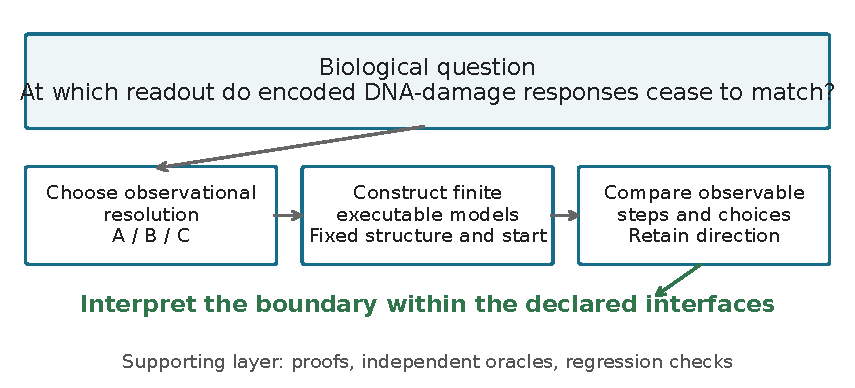
\includegraphics[width=\textwidth]{R2_Fig1.pdf}
\caption{Question-first comparison workflow. Biological readout selection
determines the observational interface before executable models are compared.
Formal verification supports the computation; the endpoint is an explicitly
model-conditional interpretation of the compatibility boundary.}
\label{fig:pipeline}
\alttext{A biological comparison question leads to readout selection, executable
models, branching comparison, and interpretation, with verification below.}
\end{figure}
